\chapter{直面配分函数}
\label{chap:18}
% Partition Function 配分函数的定义见 wiki:https://www.wikiwand.com/zh/%E9%85%8D%E5%88%86%E5%87%BD%E6%95%B0

%%%%%%%%%%%%%%%%%%%%%%%%%%%%%%%%%%%%%%%%%%%%%%%%%%%%%%%%%
%%%%%%%%%%%%%%%%%%% author:quxiaofeng %%%%%%%%%%%%%%%%%%%
%%%%%%%%%%%%%%%%%%%%%%%%%%%%%%%%%%%%%%%%%%%%%%%%%%%%%%%%%

如 \consider{16.2.2 节}中所见,很多概率模型(一般称为无向图模型)是用\consider{非标准化(unnormalized)}的概率分布 \(\widetilde{p}(\bm{x};\bm{\theta})\) 定义的。必须要用配分函数 \(Z(\bm{\theta})\) \footnote{译者注:配分函数(Partition Function)的定义见 wiki:\url{https://www.wikipedia.org/zh/\%E9\%85\%8D\%E5\%88\%86\%E5\%87\%BD\%E6\%95\%B0}} 去除 \(\widetilde{p}\) 才能得到有效的概率分布:
\begin{equation}
    p(\bm{x};\bm{\theta})
    = \frac{1}{Z(\bm{\theta})}\widetilde{p}(\bm{x};\bm{\theta}).
\end{equation}

配分函数是\consider{非标准化}概率对于所有状态的积分(连续变量)或和(离散变量): 
\begin{equation}
    \int\widetilde{p}(\bm{x})d\bm{x}
\end{equation}
 或者
 \begin{equation}
     \sum_{\bm{x}}\widetilde{p}(\bm{x}).
 \end{equation}

这个运算对于很多常用模型来说是\consider{不可解的(intractable)}。

如\consider{20 章}所见,有些深度学习模型在设计上是有可解标准化常量的,或者设计为无需计算 \(p(\bm{x})\)。但其它的模型就需要直接面对不可解配分函数的问题了。本章我们讨论训练和评估具有不可解配分函数的模型的方法。

\section{对数似然梯度}
\label{sec:18.1}

使用最大似然法学习无向模型的难点在于配分函数有参数依赖。相对参数的对数似然梯度具有与配分函数梯度相关项:
\begin{equation}
    \nabla_{\bm{\theta}}\log{p(\bm{x};\bm{\theta})}
    = \nabla_{\bm{\theta}}\log{\widetilde{p}(\bm{x};\bm{\theta})}
    - \nabla_{\bm{\theta}}\log{Z(\bm{\theta})}.
\end{equation}

这里就是著名的\consider{正相(positive phase)学习与负相(negative phase)学习}分解的产生。

对于大多数我们所关心的无向图模型,负相比较难。没有隐变量或者隐变量\consider{交互,连接}比较少的模型一般具有可解的正相。具有简单正相、复杂负相的模型的最基础的例子就是 RBM。给定可见单元,RBM 的隐单元之间条件独立。正相复杂、隐变量之间交互复杂的例子,主要集中于第 19 章。本章关注负相的复杂度。

再仔细观察一下\(\log Z\)的梯度:
\begin{align}
    & \nabla_\theta \log{Z}                                \\
    & = \frac{\nabla_\theta Z}{Z}                          \\
    & = \frac{\nabla_\theta\sum_x\widetilde{p}(\bm{x})}{Z} \\
    & = \frac{\sum_x\nabla_\theta\widetilde{p}(\bm{x})}{Z}.
\end{align}

若模型对所有 \(\bm{x}\) 都有 \(p(\bm{x})>0\),则可用 \(exp(\log\widetilde{p}(\bm{x}))\) 代换 \(\widetilde{p}(\bm{x})\):
\begin{align}
& \frac{\sum_x\nabla_\theta\exp(
	\log{\widetilde{p}(\bm{x})})}{Z}             \\
& = \frac{\sum_x\exp(\log{\widetilde{p}(\bm{x})})
	\nabla_\theta\log{\widetilde{p}(\bm{x})}}{Z} \\
& = \frac{\sum_x\widetilde{p}(\bm{x})
	\nabla_\theta\log\widetilde{p}(\bm{x})}{Z}   \\
& = \sum_{\bm{x}}p(\bm{x})
	\nabla_\theta\log\widetilde{p}(\bm{x})       \\
& = \mathbb{E}_{x\sim{}p(\bm{x})}
	\nabla_\theta\log\widetilde{p}(\bm{x}).
\end{align}

这个推导利用了离散 \(\bm{x}\) 的求和。对于连续的 \(\bm{x}\),利用积分也可以得到相似的结果。在连续版的推导中,可以使用积分号下的莱布尼茨法则得到同样的结果
\begin{equation}
    \nabla_{\bm{\theta}}\int\widetilde{p}(\bm{x})d\bm{x}
    = \int\nabla_{\bm\theta}\widetilde{p}(\bm{x})d\bm{x}.
\end{equation}
这一等同的结果只是在 \( \widetilde{p} \) 和 \( \nabla_{\bm\theta}\widetilde{p}(\bm{x})d\bm{x} \) 满足一定的正则化条件时成立。根据测度论,需要满足如下条件:(i) 非正态分布\( \widetilde{p} \) 对每一个 \(\bm{\theta}\)都是 \(\bm{x}\) 的勒贝格可积函数;(ii) 梯度 \( \nabla_{\bm\theta}\widetilde{p}(\bm{x}) \) 必须对所有 \(\bm\theta\) 和几乎所有 \(\bm x\) 都存在;(iii) 必须存在一个 \( \nabla_{\bm\theta}\widetilde{p}(\bm{x}) \) \consider{的可积确界函数} \(R({\bm x})\),使得 \(\max_i|\frac{\partial}{\partial \theta_i}\widetilde{p}(\bm{x})| \leq R(\bm{x}) \) 对所有 \(\bm\theta\) 和几乎所有 \(\bm x\) 都成立。幸好,常见机器学习模型都具有这些性质。

这种一致性
\begin{equation}\label{eqn:18.15}
    \nabla_{\bm{x}}\log{}Z
    = \mathbb{E}_{\bm{x}\sim{}p(\bm{x})}
    \nabla_{\bm{\theta}}\log\widetilde{p}(\bm{x})
\end{equation}
是蒙特卡洛方法经过适当改进后可以近似地求得配分函数可解模型的最大似然的基础。

学习无向图模型的蒙特卡洛方法为我们提供了直观的框架,可以同时考虑正相和负相。正相,根据从数据中提取的 \(\bm x\) 提高 \(\log\widetilde{p}(\bm x)\)。负相,根据模型分布降低配分函数降低 \(\log\widetilde{p}(\bm x)\)。

在深度学习文献中,一般把 \(\log\widetilde{p}\) \consider{参数化(parameterize)}为能量函数\consider{(公式 16.7)}。
这里,我们可以把正相解释为压低训练样本的能量;把负相解释为抬高模型中央本的能量,参见图~\ref{fig:18.1}。

\section{随机最大似然和对比分歧}
\label{sec:18.2}

实现公式~\ref{eqn:18.15} 的一个简单方法,是每次需要梯度的时候,预热一组随机初始化的马尔可夫链,再进行计算。使用随机梯度下降进行学习时,每次计算梯度马尔可夫链都要预热。此方法的训练过程如算法~\ref{alg:18.1} 所示。该方法在内循环中预热马尔可夫链,运算过于复杂,但为更为实际的算法提供了基准。

\begin{algorithm}
\DontPrintSemicolon
设置 \(\epsilon\),步长,应设为较小正数。\;
设置 \(k\),吉布斯(Gibbs)步长,设置时应考虑为预热(burn in)提供冗余,设置一个较大的值。在一个小图像块上训练 RBM 大约可以设为 100。\;
\While{未收敛}{
    从训练集中抽样一个包含 \(m\) 个样本 \(\{\bm{x}^{(1)},\ldots,\bm{x}^{(m)}\}\) 的小批(minibatch)\;
    \(\bm{g} \longleftarrow \frac{1}{m}\sum^m_{i=1}
    	\nabla_{\bm{\theta}}\log\widetilde{p}(\bm{x}^{(i)};\bm{\theta})\).\;
    用随机数初始化一组 \(m\) 个样本 \(\{\widetilde{\bm{x}}^{(1)},\ldots,\widetilde{\bm{x}}^{(m)}\}\)(可以使用均匀分布或正态分布,或者也可以使用与目标边缘分布相匹配的分布)。\;
    \For{\(i=1\) to \(k\)}{
    	\For{\(j=1\) to \(m\)}{
        	\(\widetilde{\bm{x}}^{(j)} 
            \longleftarrow \text{吉布斯更新}(\widetilde{\bm{x}}^{(j)}).\)\;
        }
    }
    \(\bm{g} \longleftarrow
    	\bm{g} - \frac{1}{m}\sum^m_{i=1}
    	\nabla_{\bm{\theta}}\log\widetilde{p}(\bm{x}^{(i)};\bm{\theta})\).\;
    \(\bm{\theta} \longleftarrow
    	\bm{\theta} + \epsilon\bm{g}\)\;
}
\caption{一个简单的蒙特卡洛马尔科夫链算法(MCMC)算法。利用梯度上升来计算带有可解配分函数的最大对数似然。\label{alg:18.1}}
\end{algorithm}

MCMC 求最大似然,可以看做是在两种力量中取得平衡。一方面,产生数据的地方,推高模型分布;另一方面,模型采样产生的地方压低模型分布。图~\ref{fig:18.1} 所示即为此过程。两种力量分别对应于最大化 \(\log\widetilde{p}\) 和最小化 \(\log Z\)。有几种可行的近似负相的方法。但这些近似方法都可以理解为降低负相计算复杂性的同时,在一些错误的位置压低分布。

\begin{figure}[htbp] %  figure placement: here, top, bottom, or page
   \centering
   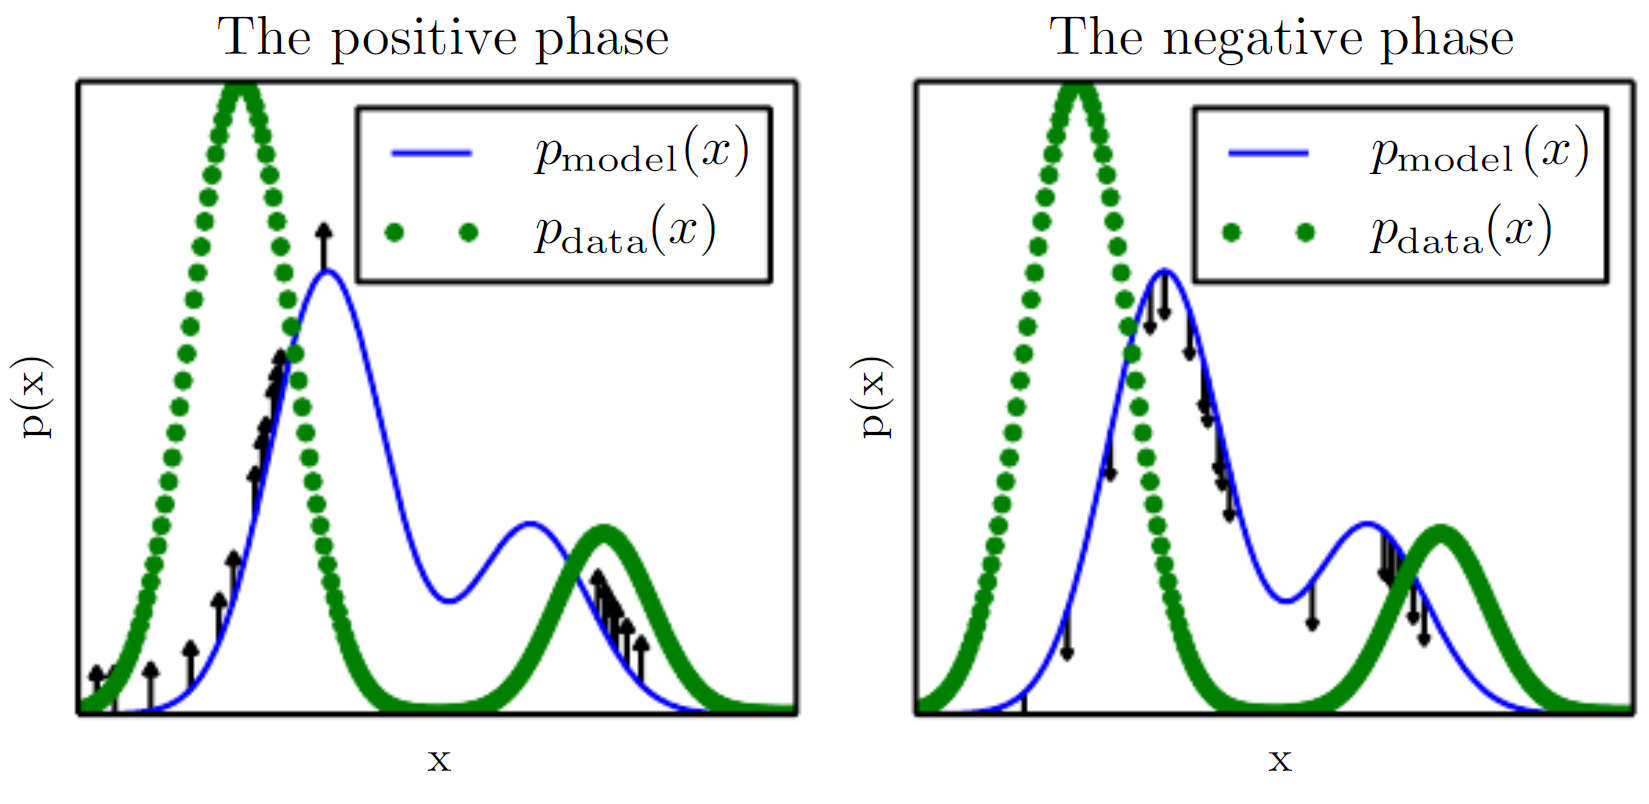
\includegraphics[width=\textwidth]{fig/chap18/18_1.png} 
   \caption{算法~\ref{alg:18.1} 的``正相''和``负相''。(左)正相时,我们从数据分布中采样一些点,然后推高非标准化的概率。数据中更有可能的点会推高得更多。(右)负相时,我们从模型中采样一些点,然后压低它们的非标准化概率。负相抵消了正相为非标准化概率在每一个位置都简单增加一个巨大常量的倾向。当数据分布和模型分布相等时,正相与负相在一点上推高和压低的几率相等。这时,梯度(的期望)就没有了,训练必然终止。}
   \label{fig:18.1}
\end{figure}

负相需要从模型分布中提取样本,这一过程开始理解为从模型中找一些非常有信心的点。
因为负相降低这些点的概率,一般认为这些是模型对世界的错误认知。
文献中一般称之为\consider{``幻象(Hallucinations)''}或\consider{``神奇粒子(Fantasy particles)''}。
其实,还真的曾有人提出负相可能是人类和其它动物做梦的原因\consider{(Circk and Mitchison, 1983)}。
其主要概念是说,大脑维护一个对于整个世界的概率模型。清醒时,当真实事件发生时,遵从 \(\log\widetilde{p}\) 的梯度;睡眠时,遵从 \(\log\widetilde{p}\) 的负梯度最小化 \(\log Z\),同时体验的则是当前模型的采样。
这个假说可以很好地解说正相和负相,他们之间的关系及其在算法中的作用,但并未被神经科学所证实。


\begin{algorithm}
\DontPrintSemicolon
设置 \(\epsilon\),步长,应设为较小正数。\;
设置 \(k\),吉布斯(Gibbs)步长,设置时,应考虑马尔可夫链从 \(p_{data}\) 中初始化时,需要从 \(p(\bm{x};\bm{\theta})\)中采样,设置为一个较大的值。在一个小图像块上训练 RBM 大约可以设为 1-20。\;
\While{未收敛}{
    从训练集中抽样一个包含 \(m\) 个样本 \(\{\bm{x}^{(1)},\ldots,\bm{x}^{(m)}\}\) 的小批(minibatch)\;
    \(\bm{g} \longleftarrow \frac{1}{m}\sum^m_{i=1}
    	\nabla_{\bm{\theta}}\log\widetilde{p}(\bm{x}^{(i)};\bm{\theta})\).\;
    \For{\(i=1\) to \(m\)}{
    	\(\widetilde{\bm{x}}^{(1)} \longleftarrow \bm{x}^{(i)}.\)\;
    }
    \For{\(i=1\) to \(k\)}{
    	\For{\(j=1\) to \(m\)}{
        	\(\widetilde{\bm{x}}^{(j)} 
            \longleftarrow \text{吉布斯更新}(\widetilde{\bm{x}}^{(j)}).\)\;
        }
    }
    \(\bm{g} \longleftarrow
    	\bm{g} - \frac{1}{m}\sum^m_{i=1}
    	\nabla_{\bm{\theta}}\log\widetilde{p}(\bm{x}^{(i)};\bm{\theta})\).\;
    \(\bm{\theta} \longleftarrow
    	\bm{\theta} + \epsilon\bm{g}.\)\;
}
\caption{对比分歧算法。利用梯度上升进行优化。\label{alg:18.2}}
\end{algorithm}

\begin{figure}[htbp] %  figure placement: here, top, bottom, or page
   \centering
   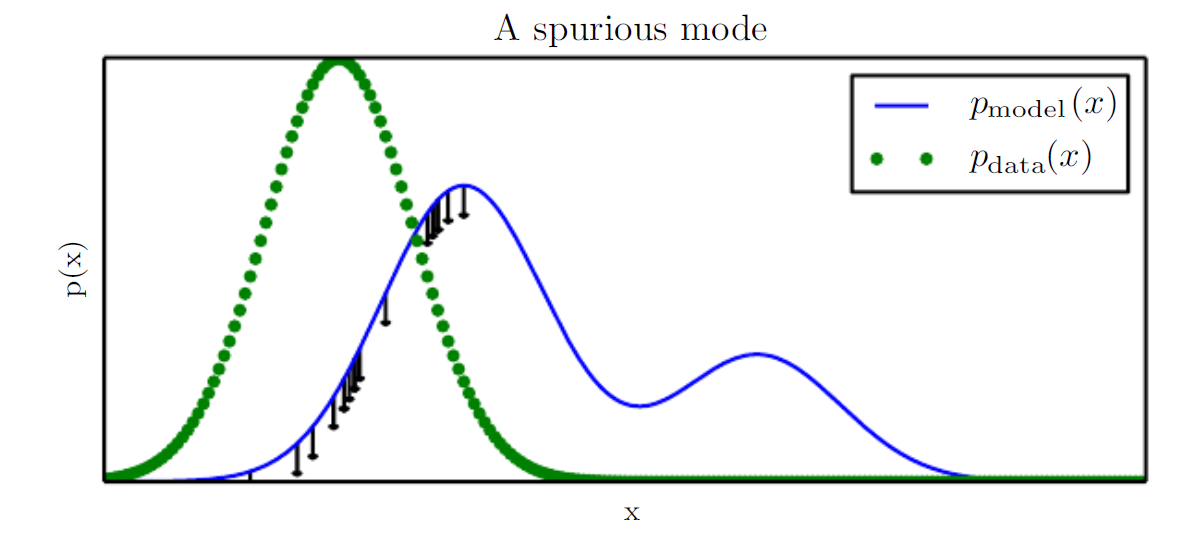
\includegraphics[width=\textwidth]{fig/chap18/18_2.png} 
   \caption{对比分歧的负相(根据算法 18.2)}
   \label{fig:18.2}
\end{figure}

\section{伪概率}
\label{sec:18.3}

\section{评分比对和比率比对}
\label{sec:18.4}

\section{评分比对的降噪}
\label{sec:18.5}

\section{噪声抑制期望}
\label{sec:18.6}

\section{配分函数期望}
\label{sec:18.7}

\subsection{基于退火算法的重要性采样}
\label{sec:18.7.1}

\subsection{桥采样}
\label{sec:18.7.2}